\documentclass{beamer}
\usetheme{Madrid}
\usepackage[utf8]{inputenc}
\usepackage{amsmath, amssymb, graphicx}
\usepackage{hyperref}
\usepackage{bm}

\title{MCBM022-23 Introdução aos Processos Estocásticos}
\subtitle{\url{professor.ufabc.edu.br/~jair.donadelli/estocastico/}}
%\author{Disciplina: Introdução a Processos Estocásticos}
\date{}

\begin{document}

\frame{\titlepage}

\begin{frame}{EMENTA}

  \begin{itemize}
  \item Cadeias de Markov discretas e comportamento assintótico:
    passeios aleatórios, processo de ramificação.
  \item Processos de Poisson. 
  \item Cadeias de Markov em tempo contínuo. 
  \item Processos de renovação. 
  \item Martingais. 
  \item Introdução ao movimento browniano.
  \end{itemize}


  \vfill

  ROSS, Sheldon M. Introduction to probability models.
  
  \vfill

  RECOMENDAÇÃO: Álgebra Linear; Cálculo de Probabilidade 
  
\end{frame}

%% ===============================================================

\begin{frame}

  \vfill
  
  3 provas, negociáveis dependendo do tamanho da turma

  \vfill
  
  Contabilizo faltas  (chamada ou lista ou QR) 

  \vfill

  Não reprovo por falta com conceito C ou maior
  
  \vfill

  Chamada ou lista,  em $\geq 13$ dias aleatórios

  \vfill
  
\end{frame}

%% ===============================================================

\begin{frame}{Motivação}
\begin{block}{Pergunta}
Como o Google decide qual página deve aparecer primeiro quando você faz uma busca?
\end{block}
\pause
\begin{itemize}
    \item Podemos modelar a web como um grafo com páginas como vértices e links como arestas.
    \item Um "robô" navega aleatoriamente pelos links da internet.
    \item A frequência com que ele visita cada página define sua importância.
\end{itemize}
\end{frame}

%% ===============================================================

\begin{frame}{Um Exemplo de Web Simples}
\begin{center}
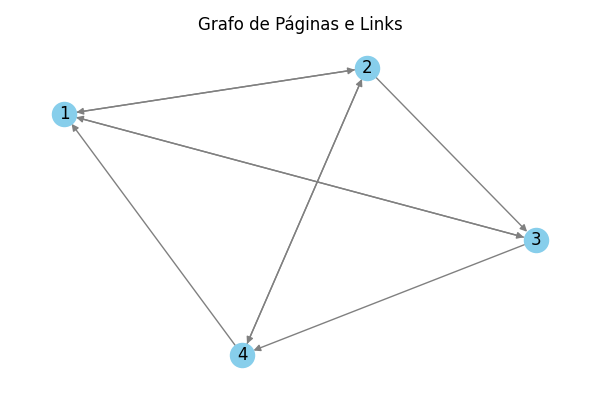
\includegraphics[width=0.7\textwidth]{web_grafo.png} \\
Grafo dirigido com 4 páginas: 1, 2, 3, 4
\end{center}
\end{frame}

%% ===============================================================

\begin{frame}{Matriz de Transição}
  \[
    P = \begin{bmatrix}
      0 & \frac{1}{2} & \frac{1}{2} & 0 \\\\
      \frac{1}{3} & 0 & \frac{1}{3} & \frac{1}{3} \\\\
      \frac{1}{2} & 0 & 0 & \frac{1}{2} \\\\
      \frac{1}{2} & \frac{1}{2} & 0 & 0
    \end{bmatrix}
  \]
  \begin{itemize}
  \item Cada linha representa uma página atual.
  \item Cada coluna representa uma página de destino.
      $$P_{ij} = \mathrm{Prob}(i\to j) = \mathbb{P} \big( X_{n+1} = j \mid X_n=i \big)$$
  \item A soma de cada linha é 1: matriz estocástica.
  \end{itemize}
  
  
\end{frame}

%% ===============================================================

\begin{frame}{Transições em 2 passos: $P^2$}
  \begin{block}{Significado de $P^2$}
    \[ (P^2)_{ij} = \mathbb{P}(X_{n+2} = j \mid X_n = i) \]
  \end{block}
  \begin{itemize}
  \item Cada entrada de $P^2$ representa a probabilidade de ir do estado $i$ para o estado $j$ em dois passos.
    \[ (P^2)_{ij} = \sum_k P_{ik} P_{kj} \]
  \item Soma sobre todos os caminhos possíveis com dois passos.
  \end{itemize}
\end{frame}

%% ===============================================================

\begin{frame}{Exemplo com a matriz $P$}
  \[ P = \begin{bmatrix}
      0 & {1}/{2} & {1}/{2} & 0 \\
      {1}/{3} & 0 & {1}/{3} & {1}/{3} \\
      {1}/{2} & 0 & 0 & {1}/{2} \\
      {1}/{2} & {1}/{2} & 0 & 0
    \end{bmatrix} \]
  \pause
  \begin{itemize}
  \item Exemplo: Qual a probabilidade de ir do estado 1 para o estado 4 em dois passos?
  \item Caminhos possíveis:
    \begin{itemize}
    \item 1 $\to$ 2 $\to$ 4: ${1}/{2} \cdot {1}/{3} = {1}/{6}$
    \item 1 $\to$ 3 $\to$ 4: ${1}/{2} \cdot {1}/{2} = {1}/{4}$
    \end{itemize}
  \item  Probabilidade ${1}/{6} + {1}/{4} = {5}/{12} \approx 0.416667$
  \end{itemize}
\end{frame}

%% ===============================================================

\begin{frame}{Em 2 passos}
  \[
    P^{\phantom{0}2} =
    \begin{bmatrix}
      0.416667 & 0       & 0.166667 & 0.416667 \\\\
      0.333333 & 0.333333 & 0.166667 & 0.166667 \\\\
      0.25     & 0.5     & 0.25     & 0        \\\\
      0.166667 & 0.25    & 0.416667 & 0.166667
    \end{bmatrix}
  \]
\end{frame}
\begin{frame}{Em 5 passos}
  \[
    P^{\phantom{0}5} =
    \begin{bmatrix}
      0.326389 & 0.263889 & 0.204861 & 0.204861 \\\\
      0.300926 & 0.270833 & 0.238426 & 0.189815 \\\\
      0.284722 & 0.260417 & 0.263889 & 0.190972 \\\\
      0.302083 & 0.211806 & 0.253472 & 0.232639
    \end{bmatrix}
\]
\end{frame}
\begin{frame}{Em 10 passos}
  \[
    P^{10} =
    \begin{bmatrix}
      0.306154 & 0.254340 & 0.235770 & 0.203736 \\\\
      0.304945 & 0.255056 & 0.237252 & 0.202747 \\\\
      0.304121 & 0.254835 & 0.238462 & 0.202582 \\\\
      0.304780 & 0.252363 & 0.238241 & 0.204616
    \end{bmatrix}
  \]
\end{frame}
\begin{frame}{Em 20 passos}
  \[
    P^{20} =
    \begin{bmatrix}
      0.305087 & 0.254236 & 0.237285 & 0.203392 \\\\
      0.305085 & 0.254239 & 0.237288 & 0.203388 \\\\
      0.305083 & 0.254240 & 0.237290 & 0.203387 \\\\
      0.305083 & 0.254234 & 0.237291 & 0.203392
    \end{bmatrix}
  \]
\end{frame}
\begin{frame}{Em 50 passos}
  \[
    P^{50} =
    \begin{bmatrix}
      0.305085 & 0.254237 & 0.237288 & 0.203390 \\\\
      0.305085 & 0.254237 & 0.237288 & 0.203390 \\\\
      0.305085 & 0.254237 & 0.237288 & 0.203390 \\\\
      0.305085 & 0.254237 & 0.237288 & 0.203390
    \end{bmatrix}
\]
\end{frame}

%% ===============================================================

\begin{frame}{Distribuição Estacionária - Resultado}
\begin{center}
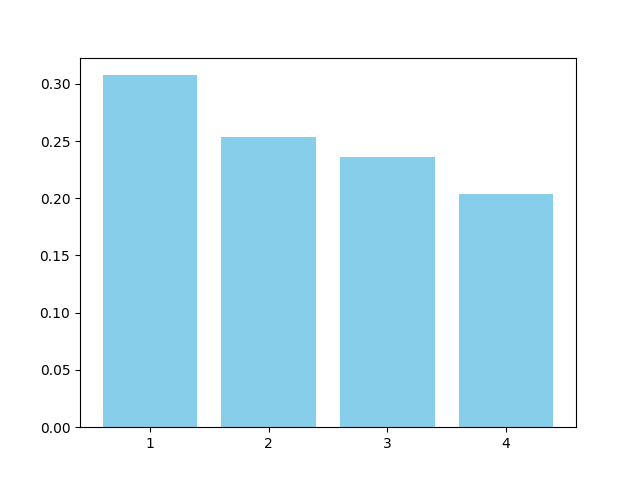
\includegraphics[width=0.65\textwidth]{stationary_dist.png} \\
Frequência de visita a cada página após 10.000 passos.
\end{center}
\end{frame}

%% ===============================================================

\begin{frame}{Simulando o "robô" do Google}
  \begin{itemize}
  \item O robô começa na página $i$ com probabilidade $\pi_i$.
  \item A cada passo, segue um link aleatório com base nas
    probabilidades da matriz.
  \item Após muitos passos, a proporção de visitas a cada página se
    estabiliza $\bm\pi_0 = (\pi_1,\dots,\pi_n) \to\bm\pi$. 
  \end{itemize}
  \begin{block}{Distribuição estacionária}
    \[ \pi P = \pi \quad \text{com} \quad \sum \pi_i = 1 \]
  \end{block}
\end{frame}

%% ===============================================================

\begin{frame}{Cálculo com Álgebra Linear}
\begin{itemize}
    \item Procuramos o vetor \( \pi \) tal que:
    \[ \bm\pi P = \bm\pi \quad \Leftrightarrow \quad (P^T - I)\bm\pi^T = \bm0 \]
    \item Isso é um problema de autovalor.
\end{itemize}
\end{frame}

%% ===========================================================================================
\end{document}


\begin{frame}{Conexões com o Curso}
\begin{itemize}
    \item Cadeias de Markov discretas: conceito central para esta aula.
    \item Processos de renovação: e se os links mudam ao longo do tempo?
    \item Martingales: a importância das expectativas condicionais.
    \item Movimento Browniano: versão contínua do passeio aleatório.
\end{itemize}
\end{frame}

\begin{frame}{Para Próximas Aulas}
\begin{itemize}
    \item Definição formal de Cadeia de Markov.
    \item Propriedades: ergodicidade, reversibilidade, estado estacionário.
    \item Exemplos com jogos, filas e processos de decisão.
\end{itemize}
\end{frame}

\begin{frame}{Referências}
\begin{itemize}
    \item Grinstead & Snell, \emph{Introduction to Probability}
    \item Norris, \emph{Markov Chains}
    \item Langville & Meyer, \emph{Google's PageRank and Beyond}
\end{itemize}
\end{frame}

\end{document}
